\documentclass[11pt]{article}
\usepackage[margin=0.85in]{geometry}
\usepackage{graphicx}
\usepackage{hyperref}
\usepackage{xcolor}
\usepackage{array}
\usepackage{enumitem}
\usepackage{parskip}
\usepackage{titlesec}
\usepackage{wrapfig}

\hypersetup{
    colorlinks=true,
    linkcolor=blue,
    urlcolor=blue,
    pdfauthor={Virinchi Addanki},
    pdftitle={Portfolio}
}

\definecolor{primary}{HTML}{1F4B99}
\definecolor{accent}{HTML}{D97706}
\definecolor{textgray}{HTML}{333333}
\definecolor{linegray}{HTML}{DDDDDD}

\titleformat{\section}
  {\Large\bfseries\color{primary}}
  {}
  {0pt}
  {}
\titlespacing*{\section}{0pt}{8pt}{6pt}

\setlength{\parskip}{6pt}
\setlength{\parindent}{0pt}
\setlist[itemize]{leftmargin=1.1em,itemsep=4pt}

\begin{document}
\pagestyle{empty}
\color{textgray}

% --- Hero --------------------------------------------------------------
\begin{minipage}[c]{0.26\textwidth}
  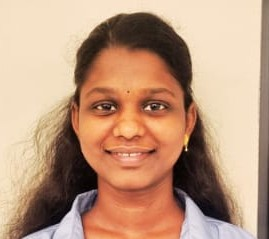
\includegraphics[width=\linewidth]{assets/profile.jpeg}
\end{minipage}
\hfill
\begin{minipage}[c]{0.7\textwidth}
  {\huge\bfseries Virinchi Addanki}\\[4pt]
  {\large Data \& Automation Engineer}\\[6pt]
  Hyderabad, India\\[6pt]
  \textcolor{primary}{\href{mailto:virinchiaddanki@gmail.com}{virinchiaddanki@gmail.com}} \quad|\quad
  +91 6300906085\\[4pt]
  \href{https://www.linkedin.com/in/virinchi-addanki/}{LinkedIn} \quad|\quad
  \href{https://github.com/addanki-virinchi}{GitHub}
\end{minipage}

\vspace{0.5cm}
\textcolor{linegray}{\rule{\textwidth}{0.6pt}}

% --- Snapshot ----------------------------------------------------------
\section*{Snapshot}
Full-stack automation and data engineer focused on production-grade web scraping, ETL, and cloud deployment. I build reliable bots for dynamic, JavaScript-heavy sites, move them to the cloud, and deliver validated datasets that people can trust.

% --- Highlights --------------------------------------------------------
\section*{Recent Highlights}
\begin{itemize}
  \item Shipped booking bots that cut manual shift scheduling by 70\% and now run on GCP (Compute Engine + GKE) with cron-driven windows.
  \item Co-created VocalLocal: AI voice platform that records, transcribes, and translates in 20+ languages; integrated ChatGPT, Gemini, and Stripe.
  \item Built multi-source scrapers (LinkedIn, Upwork, Google Maps, niche hiring sites) processing 400{,}000+ rows with validation-first pipelines.
\end{itemize}

% --- Core Skills -------------------------------------------------------
\section*{Core Skills}
\begin{itemize}
  \item Python for automation, Selenium \& Playwright for complex sites, BeautifulSoup for light parsers.
  \item ETL \& data shaping with Pandas/NumPy; exporting clean CSV/Sheets for BI teams.
  \item Cloud ops: GCP Compute Engine, Kubernetes (GKE), Instance Scheduler, CI/CD with GitHub Actions.
  \item Product-facing glue: Django, basic JS/HTML/CSS, Firebase, Stripe, OpenAI/Gemini APIs.
  \item Databases: MySQL, MongoDB; disciplined logging, retries, and error budgets.
\end{itemize}

% --- Featured Work -----------------------------------------------------
\section*{Featured Work}
\textbf{BotRecruit \quad|\quad Software Engineer \quad|\quad Jan 2025 -- Jan 2026}\\
GCP-hosted automation that books nurses' shifts with near-100\% on-time execution. Added validation layers that reduced human error by 90\%.

\vspace{6pt}
\textbf{VocalLocal \quad|\quad Python Engineer (Freelance) \quad|\quad Sep 2024 -- Feb 2025}\\
Full-stack build (Django + JS + Firebase) for AI-powered recording, transcription, and translation across 20+ languages. Payments via Stripe; LLM features via ChatGPT and Gemini. Live at \href{https://vocallocal.net/}{vocallocal.net}.

\vspace{6pt}
\textbf{Lead Pipelines \quad|\quad Freelance Data Engineer \quad|\quad Sep 2024 -- Present}\\
Country-scale scrapers for Google Maps, LinkedIn, and industry-specific job boards. Delivered normalized datasets (400k+ rows) that increased outreach efficiency by 80\%.

% --- Projects ----------------------------------------------------------
\section*{Projects}
\begin{itemize}
  \item \textbf{Google Maps Business Scraper}: extracts names, sites, phones, addresses, ratings, and review counts; two-stage pipeline (discovery + details).
  \item \textbf{Country-Level Multithreaded Scraper}: concurrent workers with logging and retry controls to cut runtime while keeping data quality high.
\end{itemize}

% --- Credentials -------------------------------------------------------
\section*{Credentials}
\begin{itemize}
  \item SQL Bootcamp (Udemy) --- \href{https://www.udemy.com/certificate/UC-d3b76d22-69b1-45dc-86fd-7a969b920a5e/}{Certificate}
  \item SQL (Intermediate) --- HackerRank \href{https://www.hackerrank.com/certificates/4e195a7134d8}{Certificate}
\end{itemize}

% --- Contact -----------------------------------------------------------
\section*{Contact}
Want a dependable scraping or automation pipeline? Drop a note at \href{mailto:virinchiaddanki@gmail.com}{virinchiaddanki@gmail.com} with the target site and desired output format. I can ship a proof-of-concept in days, harden it for production, and deploy it on GCP or your infra.

\end{document}
